\documentclass{article}
\usepackage{graphicx} % Required for inserting images
\usepackage{amsmath}
\usepackage{algorithm}
\usepackage{algorithmic}
\usepackage{listings}
\usepackage{pdfpages}
\usepackage{placeins}

\title{760-Heuristics-Assignment}
\author{Leo Mooney}
\date{March 2023}

\begin{document}
\maketitle

\section{Question 1}
Neighbors of the current solution can be found by swapping one pot in
any crucible with a pot in any other crucible.
This can be formally defined as following:

$N(\mathbf{x}) = \{\mathbf{y}(\mathbf{x}, k, l, m, n), k=1,2,3,...,16, 
l=k+1,k+2,k+3,...17, m=1,2,3, n=1,2,3\}$ where

$$\mathbf{y}(\mathbf{x},k,l,m,n)=(y_{1, 1},y_{1, 2},y_{1, 3};
y_{2, 1}y_{2, 2}y_{2, 3};...y_{c, j}),y_{c,j}=
\begin{cases}
    x_{l, n} & \text{if } c=k,j=m \\
    x_{k, m} & \text{if } c=l,j=n \\
    x_{c,j} & \text{otherwise}
\end{cases}$$

\clearpage
\section{Question 2}
Let $h(x_c) = g(\overline{Al}[x_{c,avg}], \overline{Fe}[x_{c,avg}], \overline{Si}[x_{c, avg}])$ where \\\\
$\overline{Al}[x_{c,avg}] = \displaystyle\frac{Al[x_{c,1}], Al[x_{c,2}], Al[x_{c,3}]}{3}$\\\\
$\overline{Fe}[x_{c,avg}] = \displaystyle\frac{Fe[x_{c,1}], Fe[x_{c,2}], Fe[x_{c,3}]}{3}$\\\\
$\overline{Si}[x_{c,avg}] = \displaystyle\frac{Si[x_{c,1}], Si[x_{c,2}], Si[x_{c,3}]}{3}$

\begin{algorithm}
\caption{Sweep x}
\begin{algorithmic}
  \STATE Let $S$ contain all possible solutions of $x$
  \STATE Let $x$, $x \in S$, be some initial configuration
  \STATE Let $x^*$ be some configuration that maximizes f(x)
  \STATE Let $I$ be the intermediate values\\
  \STATE $I_i := h(x_i) \forall i \in c$ 
  \WHILE {not stopped}
    \STATE Compare each neighbor $y(x, k, l, m, n) \in  N(x)$
    \STATE Let $d = h(y_k) + h(y_l) - I_k - I_l$
    \IF {$d > 0$ for some $y \in N(x)$}
      \STATE x := y
      \STATE $I_k := h(y_k)$ 
      \STATE $I_l := h(y_l)$ 
    \ELSIF {$d \le 0 \forall y \in N(x)$}
      \STATE Stop
    \ENDIF
  \ENDWHILE
  \STATE $x^* := x$
\end{algorithmic}
\end{algorithm}

\section{Question 3}
See Appendix A for all code and plots. 

\subsection{Question 3E}
Best solution found using repeated 
next ascents with $n=200$.
\begin{verbatim}
 1 [27  4 45 ] 99.261 %Al, 0.274 %Fe, 0.110 %Si, $41.53, spread = 41
 2 [ 8 13 37 ] 99.508 %Al, 0.154 %Fe, 0.153 %Si, $48.71, spread = 29
 3 [50 40 30 ] 99.504 %Al, 0.143 %Fe, 0.238 %Si, $48.71, spread = 20
 4 [17 51 15 ] 99.268 %Al, 0.162 %Fe, 0.386 %Si, $41.53, spread = 36
 5 [24 23 46 ] 99.512 %Al, 0.053 %Fe, 0.180 %Si, $48.71, spread = 23
 6 [28 12 32 ] 99.358 %Al, 0.096 %Fe, 0.348 %Si, $44.53, spread = 20
 7 [18  3 42 ] 99.760 %Al, 0.040 %Fe, 0.139 %Si, $57.35, spread = 39
 8 [19 41 20 ] 99.262 %Al, 0.212 %Fe, 0.249 %Si, $41.53, spread = 22
 9 [11 25  5 ] 99.353 %Al, 0.185 %Fe, 0.325 %Si, $44.53, spread = 20
10 [ 9  6 21 ] 99.504 %Al, 0.139 %Fe, 0.253 %Si, $48.71, spread = 15
11 [ 7 36 26 ] 99.506 %Al, 0.098 %Fe, 0.268 %Si, $48.71, spread = 29
12 [47 39  2 ] 99.503 %Al, 0.114 %Fe, 0.270 %Si, $48.71, spread = 45
13 [22 33 10 ] 99.356 %Al, 0.187 %Fe, 0.219 %Si, $44.53, spread = 23
14 [34 29 38 ] 99.361 %Al, 0.209 %Fe, 0.241 %Si, $44.53, spread =  9
15 [14 43 49 ] 99.254 %Al, 0.224 %Fe, 0.307 %Si, $41.53, spread = 35
16 [ 1 35 31 ] 99.350 %Al, 0.075 %Fe, 0.336 %Si, $44.53, spread = 34
17 [48 44 16 ] 99.515 %Al, 0.143 %Fe, 0.241 %Si, $48.71, spread = 32
                                          Sum = $787.09, MxSprd = 45
\end{verbatim}
Best solution found using repeated steepest ascents with $n=200$.
\begin{verbatim}
 1 [ 1 48 15 ] 99.256 %Al, 0.121 %Fe, 0.300 %Si, $41.53, spread = 47
 2 [29 36 10 ] 99.369 %Al, 0.216 %Fe, 0.272 %Si, $44.53, spread = 26
 3 [33  6 34 ] 99.268 %Al, 0.253 %Fe, 0.272 %Si, $41.53, spread = 28
 4 [42 16 49 ] 99.502 %Al, 0.161 %Fe, 0.163 %Si, $48.71, spread = 33
 5 [43 24 39 ] 99.508 %Al, 0.067 %Fe, 0.243 %Si, $48.71, spread = 19
 6 [47  8  5 ] 99.366 %Al, 0.188 %Fe, 0.317 %Si, $44.53, spread = 42
 7 [ 4 26 19 ] 99.253 %Al, 0.243 %Fe, 0.283 %Si, $41.53, spread = 22
 8 [31 28 46 ] 99.365 %Al, 0.139 %Fe, 0.196 %Si, $44.53, spread = 18
 9 [ 3 11 23 ] 99.502 %Al, 0.058 %Fe, 0.246 %Si, $48.71, spread = 20
10 [32 27 35 ] 99.501 %Al, 0.087 %Fe, 0.224 %Si, $48.71, spread =  8
11 [22 40 51 ] 99.353 %Al, 0.122 %Fe, 0.349 %Si, $44.53, spread = 29
12 [13 38  2 ] 99.504 %Al, 0.177 %Fe, 0.160 %Si, $48.71, spread = 36
13 [50 25 37 ] 99.500 %Al, 0.188 %Fe, 0.231 %Si, $48.71, spread = 25
14 [20 30 17 ] 99.522 %Al, 0.111 %Fe, 0.277 %Si, $48.71, spread = 13
15 [ 9 18 44 ] 99.750 %Al, 0.037 %Fe, 0.099 %Si, $57.35, spread = 35
16 [45 41 12 ] 99.258 %Al, 0.171 %Fe, 0.284 %Si, $41.53, spread = 33
17 [21  7 14 ] 99.360 %Al, 0.168 %Fe, 0.347 %Si, $44.53, spread = 14
                                          Sum = $787.09, MxSprd = 47
\end{verbatim}

\section{Quesion 4}
There does not seem to be a significant difference in the objective
value for next and steepest ascent. Steepest ascent also took far
longer to converge on each local optimum. This means that fastest
ascent is better than steepest ascent; however, this conclusion is from
limited information so it not conclusive evidence.

\section{Question 5}
(a) You would expect the problem's objective function to have lots of 
plateus because the objective function is not continuous. This means
there will be lots of cases where two pots are swapped and the
quality, and thus value, will remain constant.\\\\

\noindent (b) The best outcome is when the crucible is just above
the min/max requirements to enter the grade boundary. This is because
when sitting too far above the grade boundary there are wasted
resources (i.e. the quality doesn't need to be that good).
The proposed function will add a non-linear gradient to the existing
value function to encourage sitting on the grade boundary. This 
non-linear gradient will take the form of a quadratic with a local
minimum at the current grade boundary. The maximum value this
quadratic will take will be 1 at the next grade boundary and the 
minimum 0. This can be formally defined as follows

\[
  g'(\overline{Al}, \overline{Fe}, \overline{Si}) = 
  g(\overline{Al}, \overline{Fe}, \overline{Si})
  + \displaystyle\frac{(p-r)^2}{(q-r)^2}
\]

Where\\
$p$ is which of $\overline{Al}, \overline{Fe}, \overline{Si}$ is
closest to the current grade min/max requirement.\\
$r$ is the current grade min/max requirement for $p$.\\
$q$ is the next highest grade min/max requirement for $p$.\\

The effect this will have is that there will be a gradient encouraging
neighbors to be closer to the next grade boundary. Furthermore,
neighbors that are already closer to the next grade boundary will be
further encouraged than those who are far away from the next grade 
boundary. \\

Let us consider a simplified example where the crucible only has one 
property, $Al$. If $Al > 95$ then the value is \$10. If $Al > 97$ then the
value is \$20. Now let us consider solution x with two crucibles 
$x_k, x_l$, and a neighbor y with two crucibles $y_k, y_l$. \\
$Al[x_{k,1}]=95.3,Al[x_{k,2}]=95.2,Al[x_{k,3}]=96.5,\overline{Al}[x_k]=95.67$\\
$Al[x_{l,1}]=96.8,Al[x_{l,2}]=96.9,Al[x_{l,3}]=95.4,\overline{Al}[x_l]=96.37$\\
$Al[y_{k,1}]=95.3,Al[y_{k,2}]=95.2,Al[y_{k,3}]=95.4,\overline{Al}[y_k]=95.30$\\
$Al[y_{l,1}]=96.8,Al[y_{l,2}]=96.9,Al[y_{l,3}]=96.5,\overline{Al}[y_l]=96.73$\\

In this example using the original grading function there would be no
difference between the objective value for $x$ and $y$ so the neighbor
would not be accepted in standard next/steepest ascent. However, 
accepting the new solution would likely allow a better solution to be 
found, as crucible $l$ is closer to the \$97 boundary while
$k$ is closer to the \$95 boundary, which it will not drop below without
good reason due to the sharp change in grading function $g()$ at this
boundary.\\

Using the modified $g'()$ The crucible values are as follows\\
$x_k = \$10.112225$ 
$x_l = \$10.469225$ 
$y_k = \$10.022500$ 
$y_l = \$10.748225$ \\
This results in a change of objective value of 0.189275, meaning the
better solution will be accepted. The greatest magnitude this gradient
value can take is 1, as it is stil desirable to have a steep gradient
change when changing grades. \\

\textit{Note: This new objective function with next ascent ended up
working better than simulated annealing and was used for find my best
solutions.}

\section{Question 6}
$$g''(\overline{Al}, \overline{Fe}, \overline{Si}, x_{c1}, x_{c2}, 
x_{c3}, s) =
\begin{cases}
    g(\overline{Al}, \overline{Fe}, \overline{Si}) - 20*(s_c - s) & \text{if } s_c > s \\
    g(\overline{Al}, \overline{Fe}, \overline{Si}) & \text{otherwise}
\end{cases}$$ where
$s_c = \text{max}(x_{c1}, x_{c2}, x_{c3}) - \text{min}(x_{c1}, x_{c2}, x_{c3})$


\subsection{Task 6}
See Appendix A for code.
\subsubsection{Max Spread = 6}
\begin{verbatim}
 1 [38 34 40 ] 99.371 %Al, 0.241 %Fe, 0.163 %Si, $44.53, spread =  6
 2 [17 13 19 ] 99.270 %Al, 0.297 %Fe, 0.234 %Si, $41.53, spread =  6
 3 [35 36 39 ] 99.615 %Al, 0.043 %Fe, 0.196 %Si, $48.71, spread =  4
 4 [ 6  8 10 ] 99.352 %Al, 0.257 %Fe, 0.275 %Si, $44.53, spread =  4
 5 [30 32 27 ] 99.558 %Al, 0.093 %Fe, 0.170 %Si, $48.71, spread =  5
 6 [37 42 41 ] 99.501 %Al, 0.115 %Fe, 0.198 %Si, $48.71, spread =  5
 7 [24 22 21 ] 99.532 %Al, 0.037 %Fe, 0.276 %Si, $48.71, spread =  3
 8 [33 29 28 ] 99.256 %Al, 0.151 %Fe, 0.303 %Si, $41.53, spread =  5
 9 [11 14  9 ] 99.381 %Al, 0.080 %Fe, 0.297 %Si, $44.53, spread =  5
10 [ 5  7  3 ] 99.512 %Al, 0.188 %Fe, 0.212 %Si, $48.71, spread =  4
11 [46 47 43 ] 99.359 %Al, 0.172 %Fe, 0.315 %Si, $44.53, spread =  4
12 [26 25 31 ] 99.393 %Al, 0.138 %Fe, 0.325 %Si, $44.53, spread =  6
13 [49 48 44 ] 99.511 %Al, 0.169 %Fe, 0.145 %Si, $48.71, spread =  5
14 [20 18 23 ] 99.544 %Al, 0.057 %Fe, 0.220 %Si, $48.71, spread =  5
15 [15 16 12 ] 99.369 %Al, 0.127 %Fe, 0.302 %Si, $44.53, spread =  4
16 [ 2  4  1 ] 99.356 %Al, 0.144 %Fe, 0.280 %Si, $44.53, spread =  3
17 [50 51 45 ] 99.256 %Al, 0.198 %Fe, 0.351 %Si, $41.53, spread =  6
                                          Sum = $777.27, MxSprd =  6
\end{verbatim}

\subsubsection{Max Spread = 8}
\begin{verbatim}
 1 [15 13 11 ] 99.255 %Al, 0.157 %Fe, 0.277 %Si, $41.53, spread =  4
 2 [ 2  1  4 ] 99.356 %Al, 0.144 %Fe, 0.280 %Si, $44.53, spread =  3
 3 [46 49 51 ] 99.399 %Al, 0.152 %Fe, 0.259 %Si, $44.53, spread =  5
 4 [26 19 24 ] 99.355 %Al, 0.140 %Fe, 0.305 %Si, $44.53, spread =  7
 5 [32 29 36 ] 99.509 %Al, 0.087 %Fe, 0.197 %Si, $48.71, spread =  7
 6 [34 35 33 ] 99.358 %Al, 0.156 %Fe, 0.278 %Si, $44.53, spread =  2
 7 [ 8  3 10 ] 99.527 %Al, 0.176 %Fe, 0.194 %Si, $48.71, spread =  7
 8 [48 50 44 ] 99.544 %Al, 0.129 %Fe, 0.241 %Si, $48.71, spread =  6
 9 [14  6  7 ] 99.253 %Al, 0.249 %Fe, 0.360 %Si, $41.53, spread =  8
10 [16 18 17 ] 99.542 %Al, 0.132 %Fe, 0.258 %Si, $48.71, spread =  2
11 [30 27 23 ] 99.505 %Al, 0.105 %Fe, 0.199 %Si, $48.71, spread =  7
12 [20 22 21 ] 99.516 %Al, 0.060 %Fe, 0.277 %Si, $48.71, spread =  2
13 [43 45 38 ] 99.350 %Al, 0.226 %Fe, 0.125 %Si, $44.53, spread =  7
14 [ 9  5 12 ] 99.510 %Al, 0.106 %Fe, 0.258 %Si, $48.71, spread =  7
15 [40 39 47 ] 99.378 %Al, 0.169 %Fe, 0.269 %Si, $44.53, spread =  8
16 [28 25 31 ] 99.278 %Al, 0.204 %Fe, 0.285 %Si, $41.53, spread =  6
17 [42 41 37 ] 99.501 %Al, 0.115 %Fe, 0.198 %Si, $48.71, spread =  5
                                          Sum = $781.45, MxSprd =  8
\end{verbatim}

\subsubsection{Max Spread = 11}
\begin{verbatim}
 1 [40 49 51 ] 99.301 %Al, 0.205 %Fe, 0.295 %Si, $41.53, spread = 11
 2 [35 33 34 ] 99.358 %Al, 0.156 %Fe, 0.278 %Si, $44.53, spread =  2
 3 [ 5  3  7 ] 99.512 %Al, 0.188 %Fe, 0.212 %Si, $48.71, spread =  4
 4 [29 31 28 ] 99.257 %Al, 0.160 %Fe, 0.310 %Si, $41.53, spread =  3
 5 [ 4  6  9 ] 99.386 %Al, 0.217 %Fe, 0.204 %Si, $44.53, spread =  5
 6 [36 32 26 ] 99.524 %Al, 0.048 %Fe, 0.266 %Si, $48.71, spread = 10
 7 [39 44 47 ] 99.500 %Al, 0.124 %Fe, 0.270 %Si, $48.71, spread =  8
 8 [25 18 16 ] 99.527 %Al, 0.153 %Fe, 0.256 %Si, $48.71, spread =  9
 9 [41 50 48 ] 99.351 %Al, 0.151 %Fe, 0.329 %Si, $44.53, spread =  9
10 [14 22 24 ] 99.362 %Al, 0.083 %Fe, 0.335 %Si, $44.53, spread = 10
11 [13 23 19 ] 99.251 %Al, 0.258 %Fe, 0.213 %Si, $41.53, spread = 10
12 [30 27 20 ] 99.530 %Al, 0.104 %Fe, 0.212 %Si, $48.71, spread = 10
13 [46 42 45 ] 99.502 %Al, 0.140 %Fe, 0.056 %Si, $48.71, spread =  4
14 [21 10 17 ] 99.369 %Al, 0.239 %Fe, 0.344 %Si, $44.53, spread = 11
15 [37 43 38 ] 99.519 %Al, 0.169 %Fe, 0.143 %Si, $48.71, spread =  6
16 [11 12 15 ] 99.361 %Al, 0.068 %Fe, 0.309 %Si, $44.53, spread =  4
17 [ 8  1  2 ] 99.526 %Al, 0.042 %Fe, 0.230 %Si, $48.71, spread =  7
                                          Sum = $781.45, MxSprd = 11
\end{verbatim}


\section{My Best Solutions}
These were found by using my modified objective function from Q5 in C
with next ascent. This gave slightly better results than simulated
annealing in C. I am happy to provide the code if required for the 
competition, just email me.

\subsection{No Max Spread}
\begin{verbatim}
 1 [35 23 19 ] 99.356 %Al, 0.172 %Fe, 0.239 %Si, $44.53, spread = 16
 2 [ 5 49 26 ] 99.351 %Al, 0.188 %Fe, 0.316 %Si, $44.53, spread = 44
 3 [ 6 43  7 ] 99.350 %Al, 0.235 %Fe, 0.300 %Si, $44.53, spread = 37
 4 [24 33  1 ] 99.350 %Al, 0.056 %Fe, 0.283 %Si, $44.53, spread = 32
 5 [12 48 45 ] 99.352 %Al, 0.166 %Fe, 0.235 %Si, $44.53, spread = 36
 6 [13 39 37 ] 99.500 %Al, 0.154 %Fe, 0.170 %Si, $48.71, spread = 26
 7 [17 20 34 ] 99.351 %Al, 0.201 %Fe, 0.308 %Si, $44.53, spread = 17
 8 [29 38 41 ] 99.355 %Al, 0.154 %Fe, 0.261 %Si, $44.53, spread = 12
 9 [11  2 16 ] 99.500 %Al, 0.087 %Fe, 0.272 %Si, $48.71, spread = 14
10 [47  3 15 ] 99.351 %Al, 0.172 %Fe, 0.287 %Si, $44.53, spread = 44
11 [28 50 22 ] 99.350 %Al, 0.126 %Fe, 0.329 %Si, $44.53, spread = 28
12 [51  9 36 ] 99.517 %Al, 0.070 %Fe, 0.264 %Si, $48.71, spread = 42
13 [27 25  4 ] 99.350 %Al, 0.253 %Fe, 0.204 %Si, $44.53, spread = 23
14 [14 40 46 ] 99.351 %Al, 0.173 %Fe, 0.232 %Si, $44.53, spread = 32
15 [30  8 10 ] 99.500 %Al, 0.167 %Fe, 0.227 %Si, $48.71, spread = 22
16 [21 32 31 ] 99.501 %Al, 0.089 %Fe, 0.201 %Si, $48.71, spread = 11
17 [44 42 18 ] 99.750 %Al, 0.044 %Fe, 0.136 %Si, $57.35, spread = 26
                                          Sum = $790.73, MxSprd = 44
\end{verbatim}

\subsection{Max Spread = 6}
\begin{verbatim}
 1 [44,49,48,] 99.511 %Al, 0.169 %Fe, 0.145 %Si, $48.71, spread=5
 2 [18,19,21,] 99.512 %Al, 0.163 %Fe, 0.187 %Si, $48.71, spread=3
 3 [43,47,46,] 99.359 %Al, 0.172 %Fe, 0.315 %Si, $44.53, spread=4
 4 [9,11,12,] 99.535 %Al, 0.015 %Fe, 0.265 %Si, $48.71, spread=3
 5 [27,24,22,] 99.502 %Al, 0.068 %Fe, 0.194 %Si, $48.71, spread=5
 6 [36,39,34,] 99.502 %Al, 0.139 %Fe, 0.173 %Si, $48.71, spread=5
 7 [25,23,28,] 99.267 %Al, 0.185 %Fe, 0.332 %Si, $41.53, spread=5
 8 [38,37,42,] 99.650 %Al, 0.118 %Fe, 0.067 %Si, $52.44, spread=5
 9 [51,50,45,] 99.256 %Al, 0.198 %Fe, 0.351 %Si, $41.53, spread=6
 10 [2,7,5,] 99.505 %Al, 0.182 %Fe, 0.208 %Si, $48.71, spread=5
 11 [29,26,31,] 99.372 %Al, 0.094 %Fe, 0.350 %Si, $44.53, spread=5
 12 [16,14,20,] 99.298 %Al, 0.164 %Fe, 0.379 %Si, $41.53, spread=6
 13 [33,32,30,] 99.541 %Al, 0.070 %Fe, 0.160 %Si, $48.71, spread=3
 14 [6,8,10,] 99.352 %Al, 0.257 %Fe, 0.275 %Si, $44.53, spread=4
 15 [3,1,4,] 99.363 %Al, 0.151 %Fe, 0.284 %Si, $44.53, spread=3
 16 [13,15,17,] 99.276 %Al, 0.220 %Fe, 0.261 %Si, $41.53, spread=4
 17 [35,40,41,] 99.335 %Al, 0.141 %Fe, 0.317 %Si, $41.53, spread=6
Sum = $779.18, MxSprd = 6 
\end{verbatim}
\subsection{Max Spread = 8}
\begin{verbatim}
 1 [8,1,6,] 99.358 %Al, 0.130 %Fe, 0.315 %Si, $44.53, spread=7
 2 [24,27,21,] 99.506 %Al, 0.091 %Fe, 0.245 %Si, $48.71, spread=6
 3 [26,31,29,] 99.372 %Al, 0.094 %Fe, 0.350 %Si, $44.53, spread=5
 4 [32,40,34,] 99.353 %Al, 0.199 %Fe, 0.210 %Si, $44.53, spread=8
 5 [46,44,41,] 99.507 %Al, 0.108 %Fe, 0.191 %Si, $48.71, spread=5
 6 [22,15,18,] 99.514 %Al, 0.064 %Fe, 0.164 %Si, $48.71, spread=7
 7 [17,13,20,] 99.359 %Al, 0.191 %Fe, 0.305 %Si, $44.53, spread=7
 8 [38,33,35,] 99.501 %Al, 0.105 %Fe, 0.167 %Si, $48.71, spread=5
 9 [47,39,43,] 99.370 %Al, 0.153 %Fe, 0.341 %Si, $44.53, spread=8
 10 [7,2,5,] 99.505 %Al, 0.182 %Fe, 0.208 %Si, $48.71, spread=5
 11 [51,45,50,] 99.256 %Al, 0.198 %Fe, 0.351 %Si, $41.53, spread=6
 12 [12,16,19,] 99.362 %Al, 0.204 %Fe, 0.275 %Si, $44.53, spread=7
 13 [11,9,14,] 99.381 %Al, 0.080 %Fe, 0.297 %Si, $44.53, spread=5
 14 [36,30,37,] 99.654 %Al, 0.098 %Fe, 0.129 %Si, $52.44, spread=7
 15 [10,3,4,] 99.357 %Al, 0.278 %Fe, 0.244 %Si, $44.53, spread=7
 16 [49,48,42,] 99.513 %Al, 0.147 %Fe, 0.139 %Si, $48.71, spread=7
 17 [28,25,23,] 99.267 %Al, 0.185 %Fe, 0.332 %Si, $41.53, spread=5
Sum = $784.00, MxSprd = 8      
\end{verbatim}
\subsection{Max Spread = 11}
\begin{verbatim}
 1 [49,46,51,] 99.399 %Al, 0.152 %Fe, 0.259 %Si, $44.53, spread=5
 2 [26,37,32,] 99.514 %Al, 0.072 %Fe, 0.266 %Si, $48.71, spread=11
 3 [19,21,29,] 99.356 %Al, 0.204 %Fe, 0.263 %Si, $44.53, spread=10
 4 [20,30,23,] 99.503 %Al, 0.072 %Fe, 0.255 %Si, $48.71, spread=10
 5 [25,28,36,] 99.360 %Al, 0.186 %Fe, 0.275 %Si, $44.53, spread=11
 6 [2,1,4,] 99.356 %Al, 0.144 %Fe, 0.280 %Si, $44.53, spread=3
 7 [17,16,6,] 99.354 %Al, 0.238 %Fe, 0.341 %Si, $44.53, spread=11
 8 [34,35,33,] 99.358 %Al, 0.156 %Fe, 0.278 %Si, $44.53, spread=2
 9 [45,43,38,] 99.350 %Al, 0.226 %Fe, 0.125 %Si, $44.53, spread=7
 10 [10,3,13,] 99.353 %Al, 0.271 %Fe, 0.287 %Si, $44.53, spread=10
 11 [39,44,47,] 99.500 %Al, 0.124 %Fe, 0.270 %Si, $48.71, spread=8
 12 [7,9,5,] 99.504 %Al, 0.163 %Fe, 0.166 %Si, $48.71, spread=4
 13 [42,40,31,] 99.500 %Al, 0.131 %Fe, 0.120 %Si, $48.71, spread=11
 14 [11,8,14,] 99.375 %Al, 0.082 %Fe, 0.312 %Si, $44.53, spread=6
 15 [22,27,24,] 99.502 %Al, 0.068 %Fe, 0.194 %Si, $48.71, spread=5
 16 [15,12,18,] 99.502 %Al, 0.068 %Fe, 0.241 %Si, $48.71, spread=6
 17 [48,41,50,] 99.351 %Al, 0.151 %Fe, 0.329 %Si, $44.53, spread=9
Sum = $786.27, MxSprd = 11                                                                                                                                                                                                                                           
\end{verbatim}

\section{Appendix A}
See overleaf

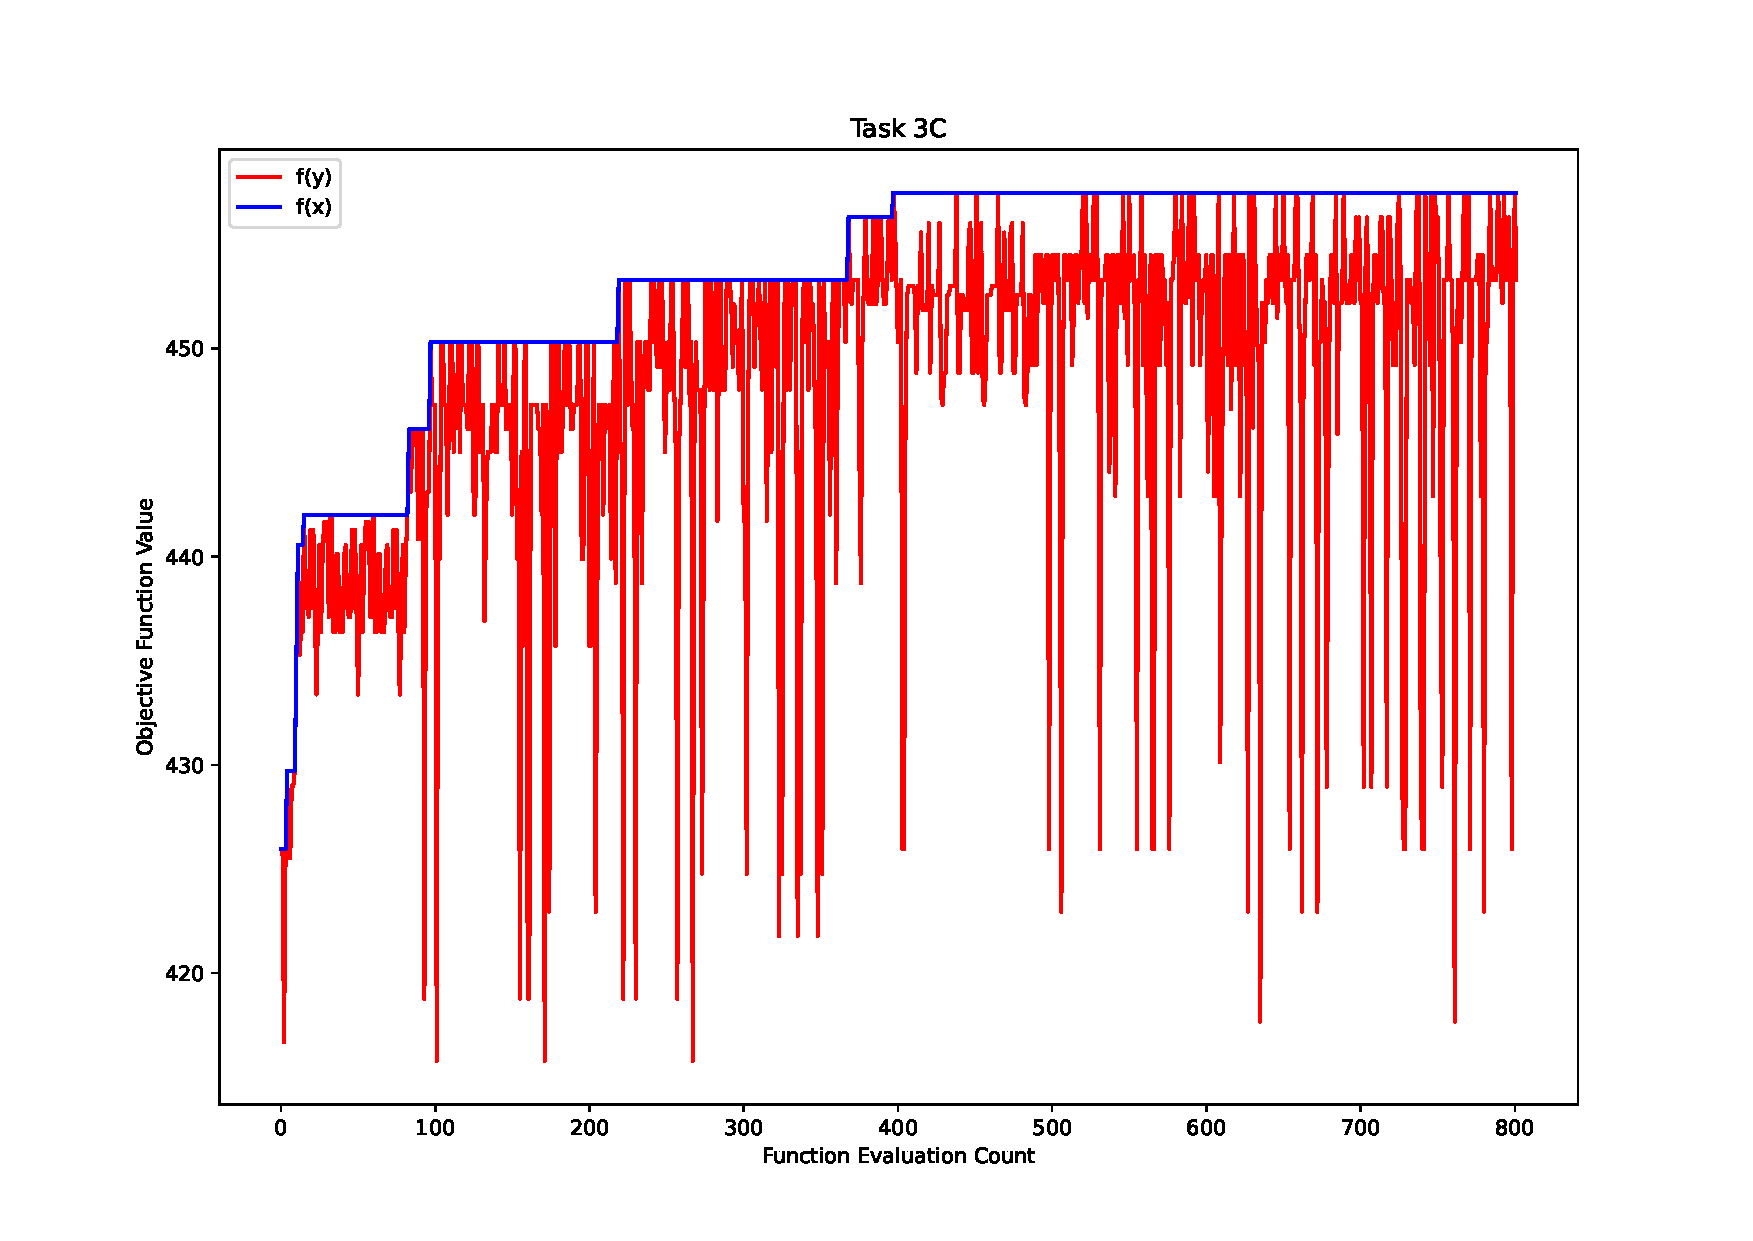
\includepdf[landscape=true,pages=-]{./assets/next_ascent_chart.pdf}
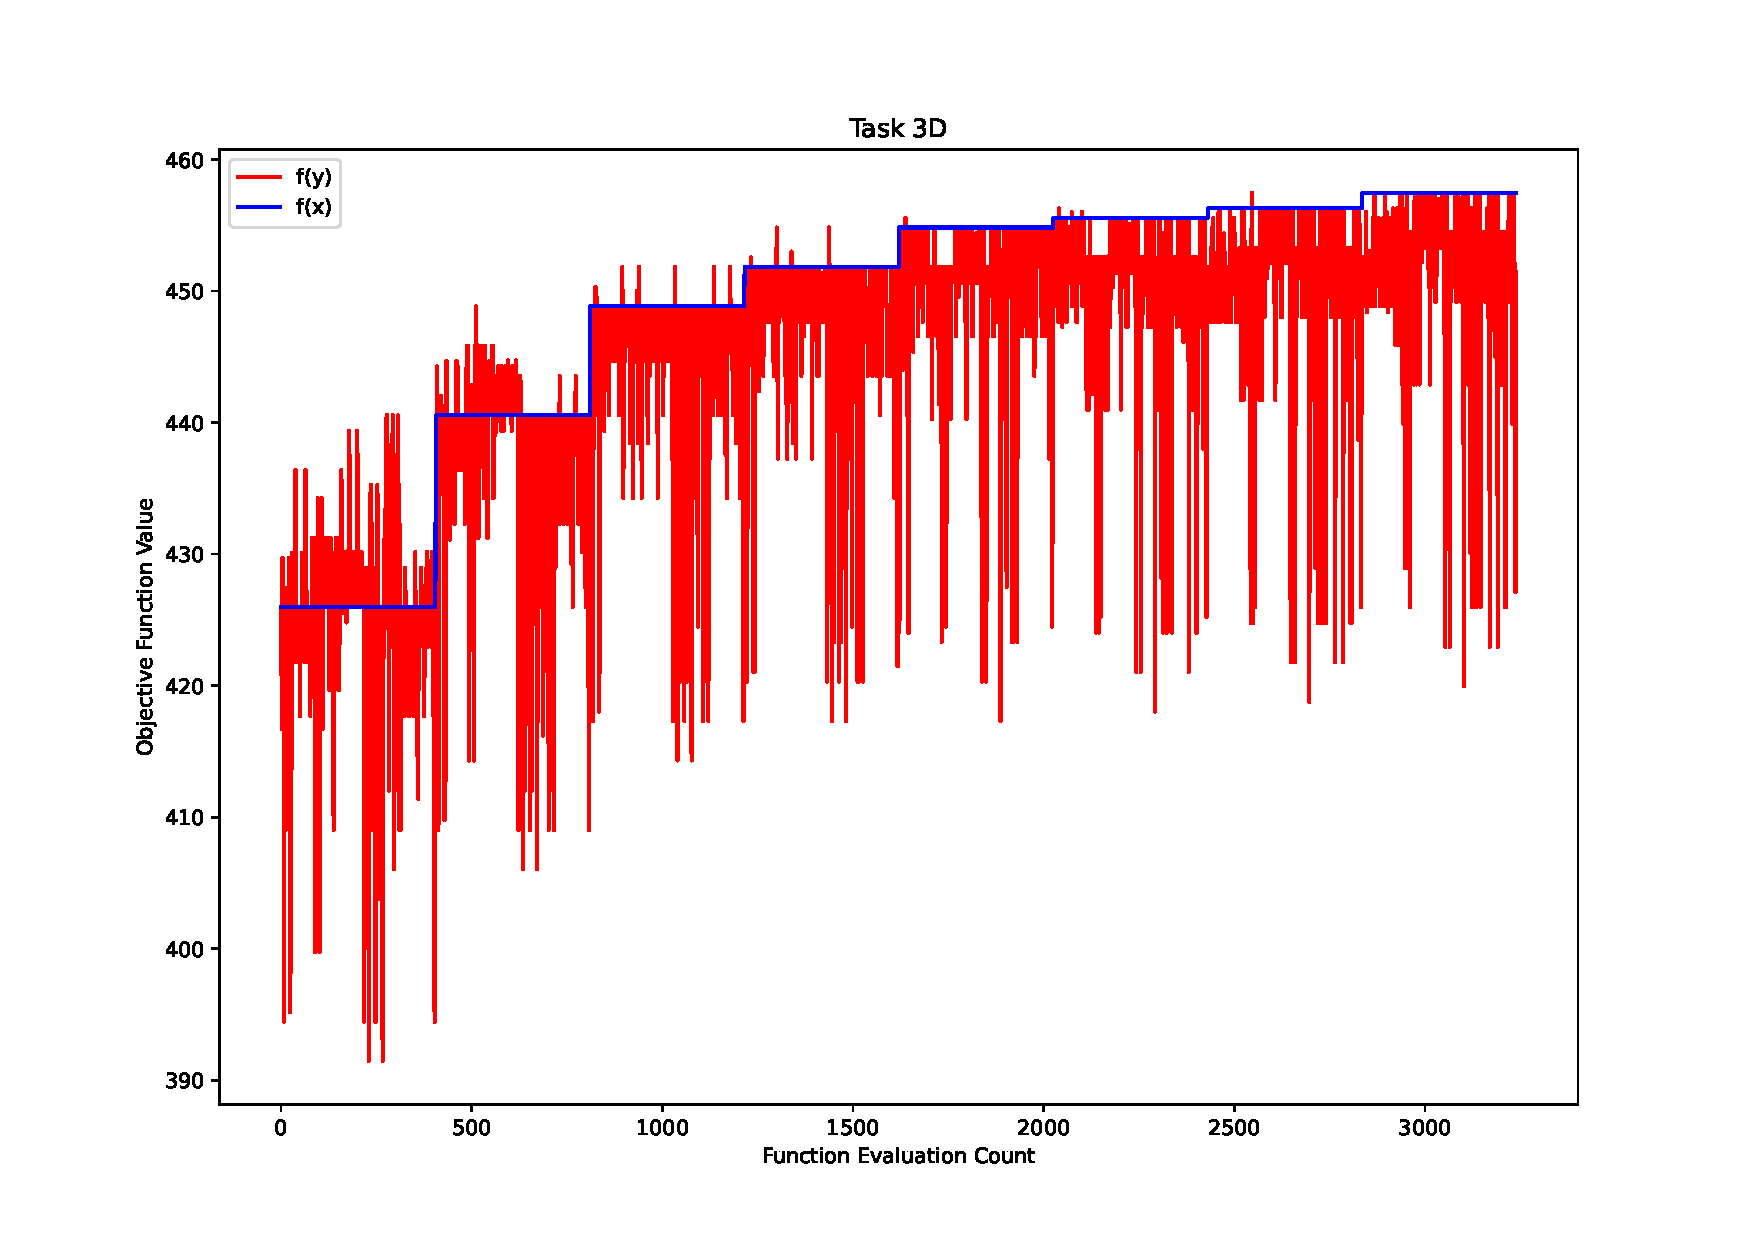
\includepdf[landscape=true,pages=-]{./assets/steepest_ascent_chart.pdf}
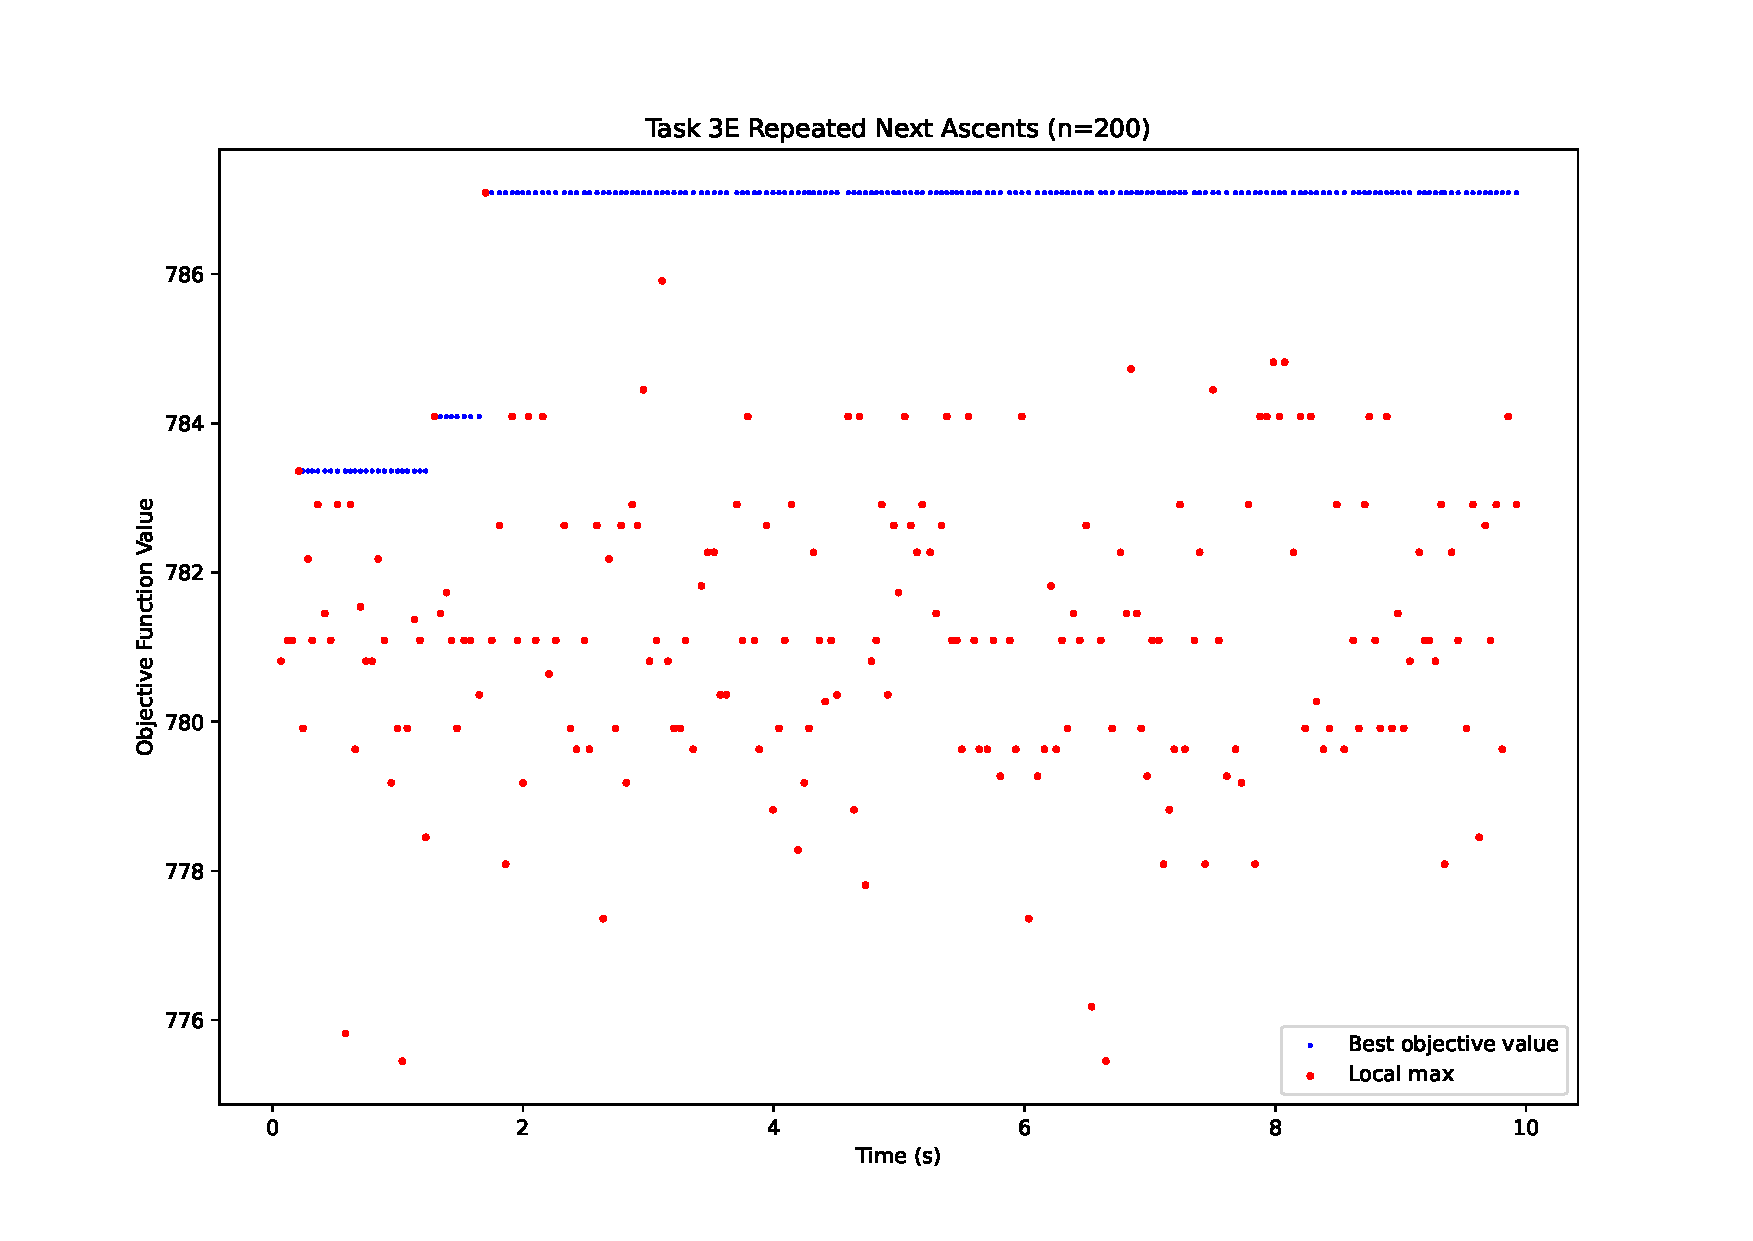
\includepdf[landscape=true,pages=-]{./assets/repeated_next_ascents_chart.pdf}
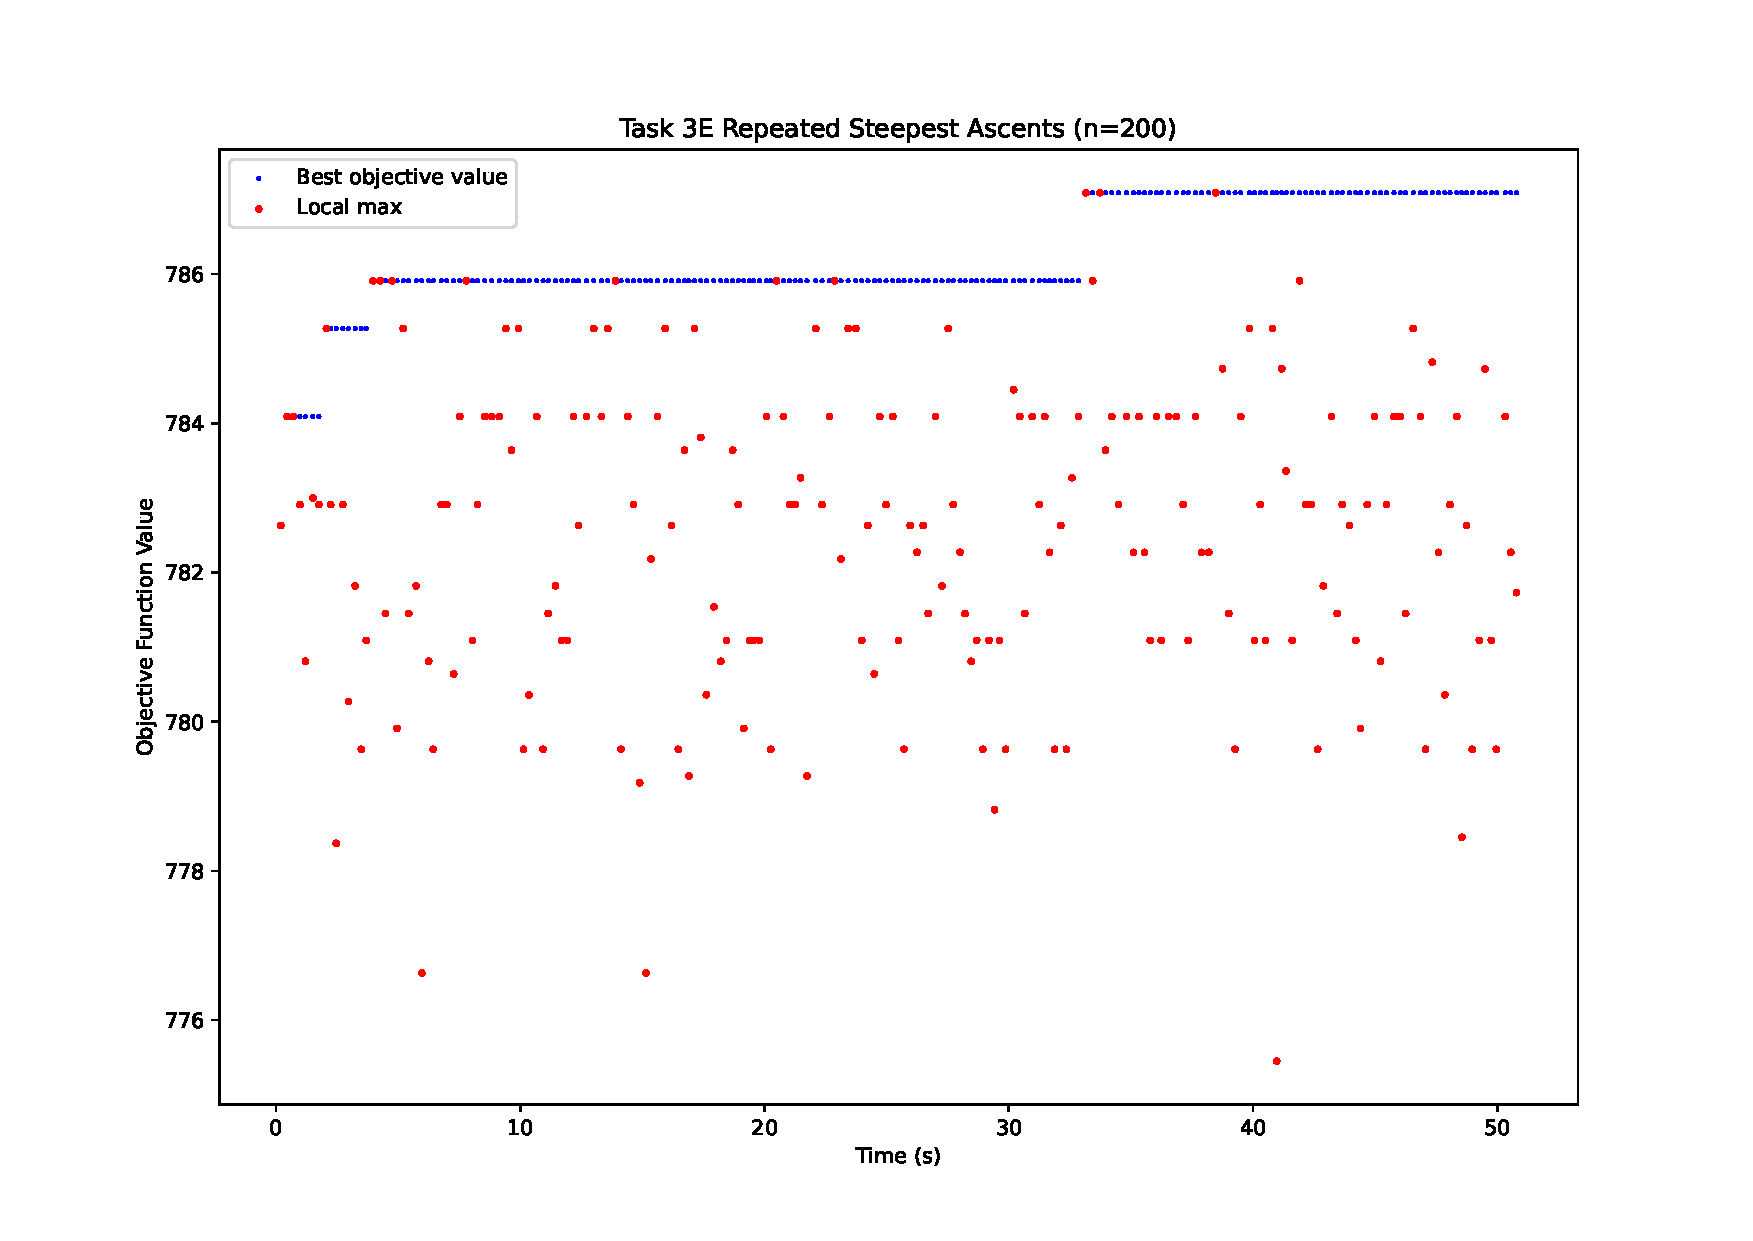
\includepdf[landscape=true,pages=-]{./assets/repeated_steepest_ascents_chart.pdf}


\end{document}
